%%%%%%%%%%%%%%%%%%%%%%%%%%%%%%%%%%%%%%%%%%%%%%%%%%%%%%%%%%%%%%%%%%%%%%%%%%%%%%%
%                       CARREGA DE LA CLASSE DE DOCUMENT                      %
%                                                                             %
% Les opcions admissibles son:                                                %
%      12pt / 11pt            (cos dels tipus de lletra; no feu servir 10pt)  %
%                                                                             %
% catalan/spanish/english     (llengua principal del treball)                 %
%                                                                             % 
% french/italian/german...    (si necessiteu fer servir alguna altra llengua) %
%                                                                             %
% listoffigures               (El document inclou un Index de figures)        %
% listoftables                (El document inclou un Index de taules)         %
% listofquadres               (El document inclou un Index de quadres)        %
% listofalgorithms            (El document inclou un Index d'algorismes)      %
%                                                                             %
%%%%%%%%%%%%%%%%%%%%%%%%%%%%%%%%%%%%%%%%%%%%%%%%%%%%%%%%%%%%%%%%%%%%%%%%%%%%%%%

\documentclass[11pt,spanish,listoffigures,listoftables]{tfgetsinf}


\usepackage{pgfplotstable} % Para leer y mostrar tablas desde CSV
\usepackage{booktabs}       % Para mejorar el diseño de la tabla
\usepackage{multirow}       % Para fusionar filas
\usepackage{caption}
\usepackage{subcaption}

\usepackage{float}          % Para usar [H] en las figuras
%%%%%%%%%%%%%%%%%%%%%%%%%%%%%%%%%%%%%%%%%%%%%%%%%%%%%%%%%%%%%%%%%%%%%%%%%%%%%%%
%                     CODIFICACIO DEL FITXER FONT                             %
%                                                                             %
%    windows fa servir normalment 'ansinew'                                   %
%    amb linux es possible que siga 'latin1' o 'latin9'                       %
%    Pero el mes recomanable es fer servir utf8 (unicode 8)                   %
%                                          (si el vostre editor ho permet)    % 
%%%%%%%%%%%%%%%%%%%%%%%%%%%%%%%%%%%%%%%%%%%%%%%%%%%%%%%%%%%%%%%%%%%%%%%%%%%%%%%

\usepackage[utf8]{inputenc} 
%%%%%%%%%%%%%%%%%%%%%%%%%%%%%%%%%%%%%%%%%%%%%%%%%%%%%%%%%%%%%%%%%%%%%
% Para conseguir que la tabla de contenido no salga en rojo
%%%%%%%%%%%%%%%%%%%%%%%%%%%%%%%%%%%%%%%%%%%%%%%%%%%%%%%%%%%%%%%%%%%%%

\hypersetup{ colorlinks=true, linkcolor=black, urlcolor=cyan, }



%%%%%%%%%%%%%%%%%%%%%%%%%%%%%%%%%%%%%%%%%%%%%%%%%%%%%%%%%%%%%%%%%%%%%%%%%%%%%%%
%                        ALTRES PAQUETS I DEFINICIONS                         %
%                                                                             %
% Carregueu aci els paquets que necessiteu i declareu les comandes i entorns  %
%                                          (aquesta seccio pot ser buida)     %
%%%%%%%%%%%%%%%%%%%%%%%%%%%%%%%%%%%%%%%%%%%%%%%%%%%%%%%%%%%%%%%%%%%%%%%%%%%%%%%



%%%%%%%%%%%%%%%%%%%%%%%%%%%%%%%%%%%%%%%%%%%%%%%%%%%%%%%%%%%%%%%%%%%%%%%%%%%%%%%
%                        DADES DEL TREBALL                                    %
%                                                                             %
% titol, alumne, tutor i curs academic                                        %
%%%%%%%%%%%%%%%%%%%%%%%%%%%%%%%%%%%%%%%%%%%%%%%%%%%%%%%%%%%%%%%%%%%%%%%%%%%%%%%

\title{Detección de defectos en objetos en movimiento mediante Redes Neuronales Convolucionales con optimizaciones específicas para hardware NVIDIA}
\author{Haro Armero, Abel}
\tutor{Flich Cardo, José}
%\tutor{López Rodríguez, Pedro Juan}
\curs{2024-2025}

%%%%%%%%%%%%%%%%%%%%%%%%%%%%%%%%%%%%%%%%%%%%%%%%%%%%%%%%%%%%%%%%%%%%%%%%%%%%%%%
%                     PARAULES CLAU/PALABRAS CLAVE/KEY WORDS                  %
%                                                                             %
% Independentment de la llengua del treball, s'hi han d'incloure              %
% les paraules clau i el resum en els tres idiomes                            %
%%%%%%%%%%%%%%%%%%%%%%%%%%%%%%%%%%%%%%%%%%%%%%%%%%%%%%%%%%%%%%%%%%%%%%%%%%%%%%%

\keywords{????, ?????????, ????, ?????????????????} % Paraules clau 
         {?????, ???, ???????????????}              % Palabras clave
         {?????, ????? ?????, ?????????????}        % Key words

%%%%%%%%%%%%%%%%%%%%%%%%%%%%%%%%%%%%%%%%%%%%%%%%%%%%%%%%%%%%%%%%%%%%%%%%%%%%%%%
%                              INICI DEL DOCUMENT                             %
%%%%%%%%%%%%%%%%%%%%%%%%%%%%%%%%%%%%%%%%%%%%%%%%%%%%%%%%%%%%%%%%%%%%%%%%%%%%%%%

\begin{document}

%%%%%%%%%%%%%%%%%%%%%%%%%%%%%%%%%%%%%%%%%%%%%%%%%%%%%%%%%%%%%%%%%%%%%%%%%%%%%%%
%              RESUMS DEL TFG EN VALENCIA, CASTELLA I ANGLES                  %
%%%%%%%%%%%%%%%%%%%%%%%%%%%%%%%%%%%%%%%%%%%%%%%%%%%%%%%%%%%%%%%%%%%%%%%%%%%%%%%

\begin{abstract}
????
\end{abstract}
\begin{abstract}[spanish]
????
\end{abstract}
\begin{abstract}[english]
????
\end{abstract}

%%%%%%%%%%%%%%%%%%%%%%%%%%%%%%%%%%%%%%%%%%%%%%%%%%%%%%%%%%%%%%%%%%%%%%%%%%%%%%%
%                              CONTINGUT DEL TREBALL                          %
%%%%%%%%%%%%%%%%%%%%%%%%%%%%%%%%%%%%%%%%%%%%%%%%%%%%%%%%%%%%%%%%%%%%%%%%%%%%%%%

\mainmatter

%%%%%%%%%%%%%%%%%%%%%%%%%%%%%%%%%%%%%%%%%%%%%%%%%%%%%%%%%%%%%%%%%%%%%%%%%%%%%%%
%                                  INTRODUCCIO                                %
%%%%%%%%%%%%%%%%%%%%%%%%%%%%%%%%%%%%%%%%%%%%%%%%%%%%%%%%%%%%%%%%%%%%%%%%%%%%%%%

\chapter{Introducci\'on}
Durante los últimos años, la inteligencia artificial ha experimentado un crecimiento en popularidad sin precedentes, transformando nuestra capacidad tecnológica con herramientas revolucionarias. Este avance ha sido impulsado por la disponibilidad de grandes volúmenes de datos y el desarrollo de algoritmos avanzados, que han permitido a las máquinas aprender y adaptarse a situaciones complejas. Algunos campos destacados de aplicación incluyen el procesamiento del lenguaje natural, la visión por computador y la robótica. En particular, la visión por computador ha visto un auge significativo, con aplicaciones en áreas como la seguridad, la medicina y la automoción. Este creciente interés se refleja en la evolución del interés público en inteligencia artificial, como muestra la Figura~\ref{fig:interes_en_inteligencia_artificial}, basada en datos de Google Trends \cite{googletrends2025}.



\begin{figure}[H]
   \centering
   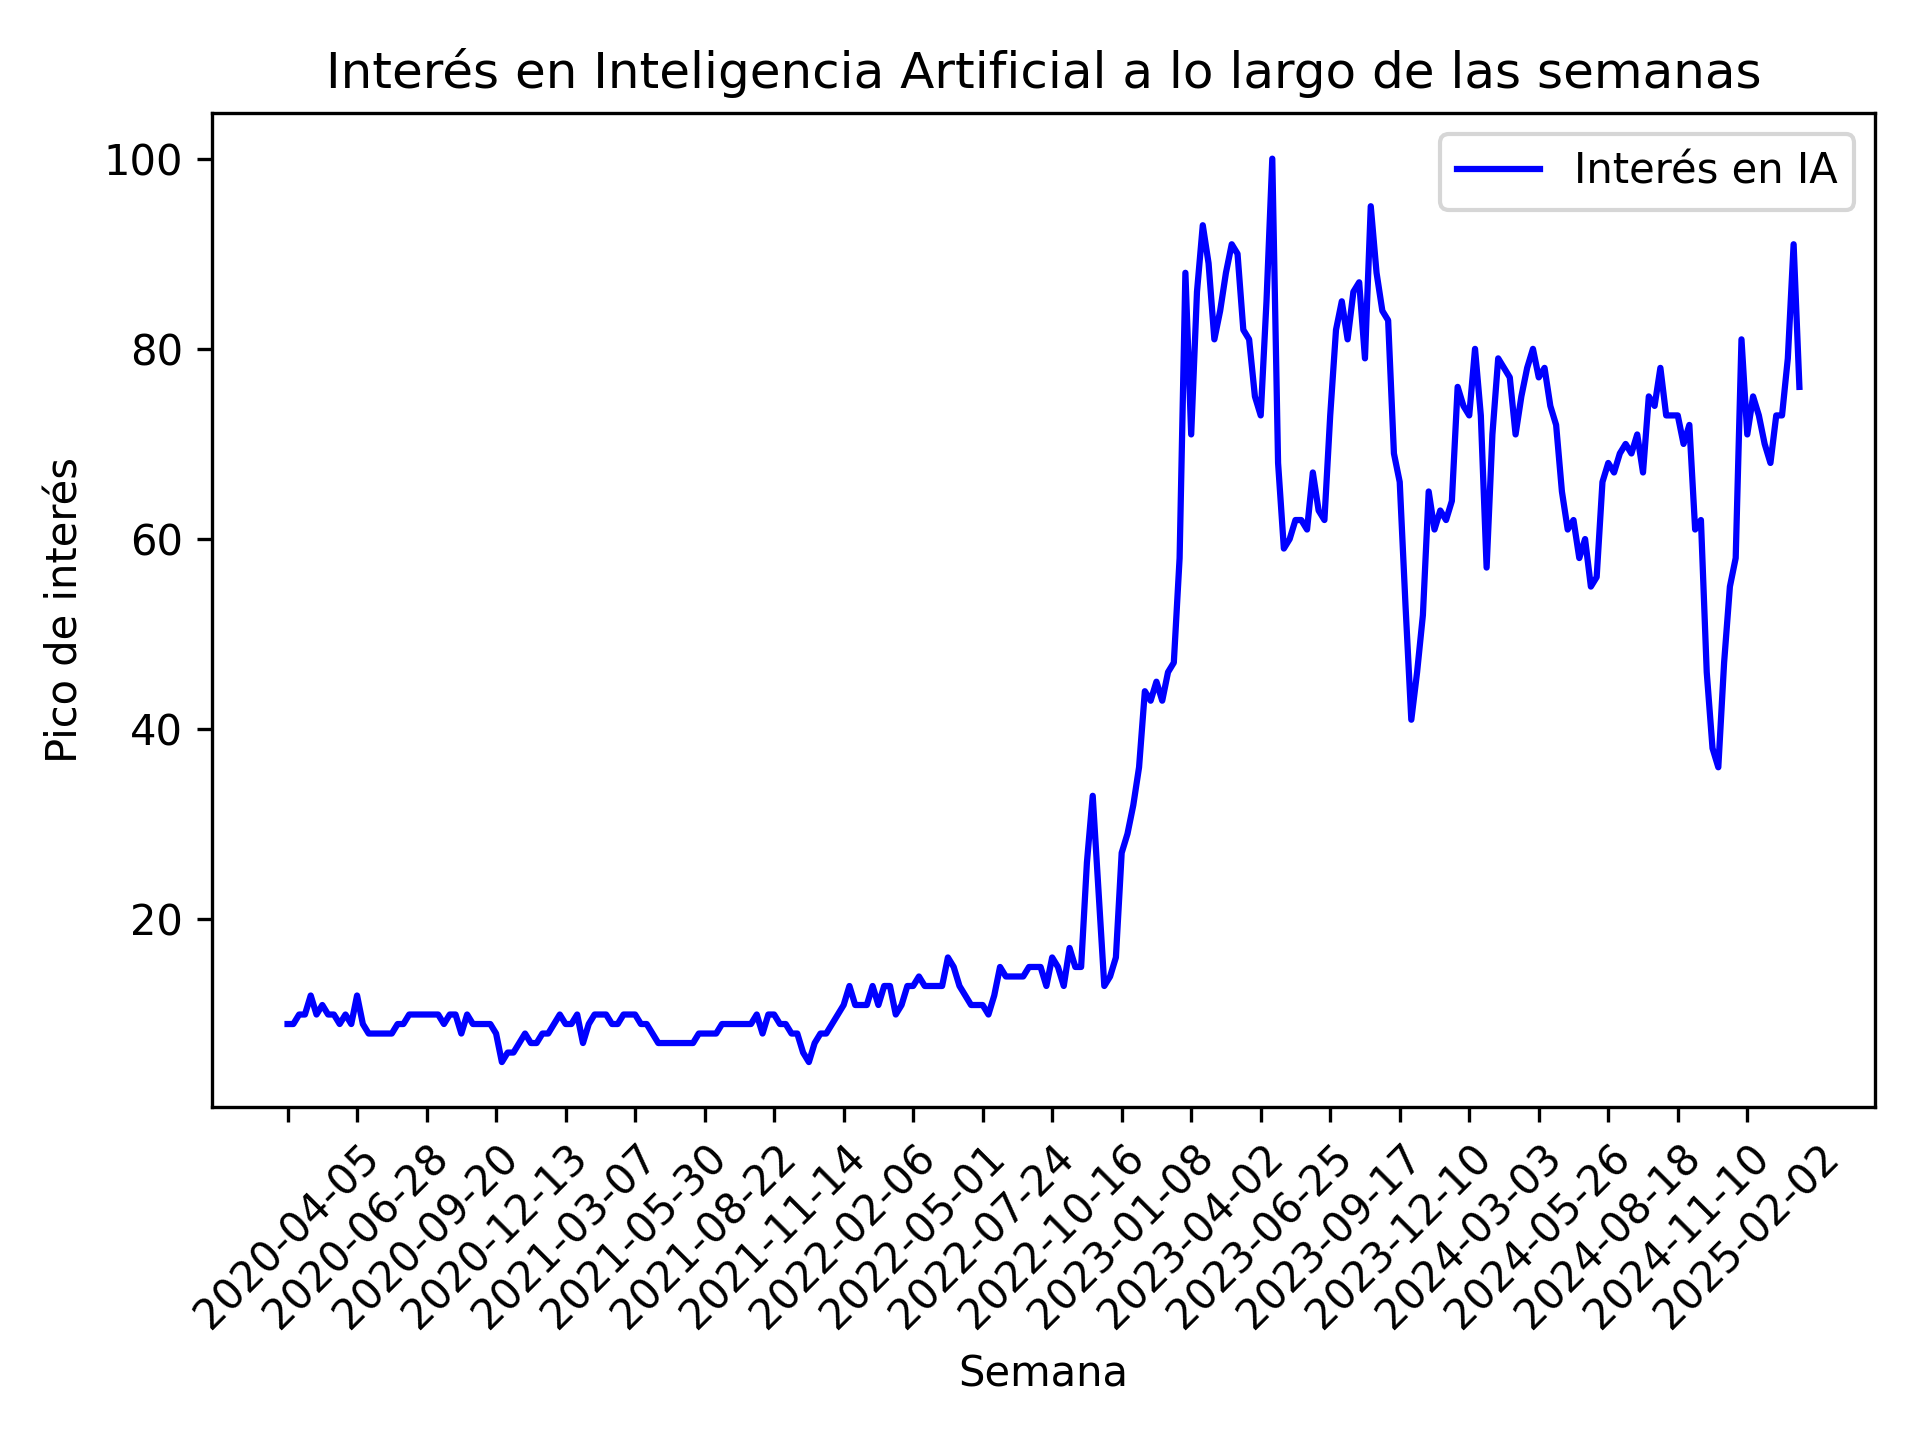
\includegraphics[width=0.7\textwidth]{excels/introduccion/interes_en_ia.png}
   \caption{Evolución del interés público en inteligencia artificial según datos de Google Trends (2020-2025)}
\label{fig:interes_en_inteligencia_artificial}
\end{figure}

Este progreso ha sido posible gracias a los avances en redes neuronales convolucionales, que han revolucionado la capacidad de los sistemas para detectar y clasificar objetos en imágenes y vídeos con una gran precisión y velocidad.

Estos algoritmos de visión artificial requieren una potencia computacional significativa tanto para su entrenamiento como para su ejecución. Las CPUs (Unidades Centrales de Procesamiento) tradicionales resultan insuficientes para estas tareas, por lo que la industria ha desarrollado arquitecturas específicas como las GPUs (Unidades de Procesamiento Gráfico), TPUs (Unidades de Procesamiento Tensorial) y DLAs (Aceleradores de Aprendizaje Profundo). Estos componentes están optimizados para ejecutar operaciones de entrenamiento e inferencia de manera eficiente, permitiendo implementar sistemas de visión artificial capaces de procesar información visual en tiempo real. Sin embargo, estos aceleradores suelen presentar un consumo energético elevado, lo que plantea importantes retos de eficiencia y sostenibilidad.


\begin{figure}[H]
   \centering
   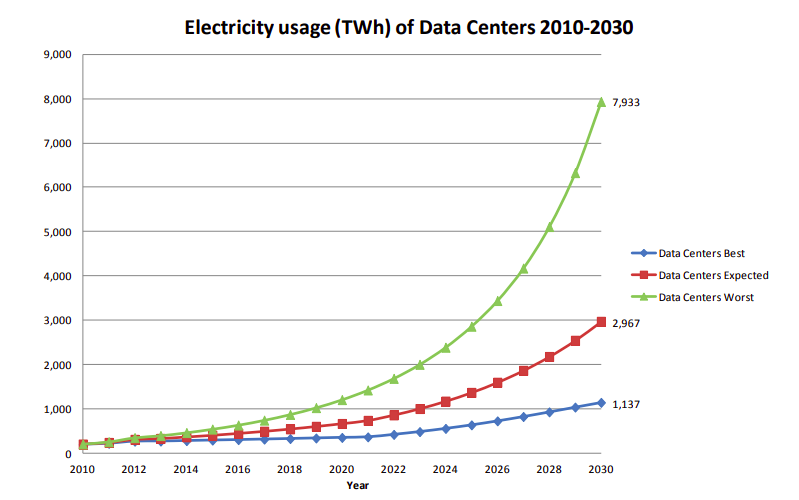
\includegraphics[width=0.7\textwidth]{images/introduccion/consumo_electrico_datacenters.png}
   \caption{Proyección del consumo eléctrico de los centros de datos en el mundo}
\label{fig:consumo_electrico_datacenters}
\end{figure}

Como se observa en la Figura~\ref{fig:consumo_electrico_datacenters}, el consumo eléctrico de los centros de datos en el mundo ha ido aumentando de forma exponencial, lo que plantea un desafío significativo para la sostenibilidad del crecimiento tecnológico \cite{challe6010117}. En el peor escenario, esta tendencia podría llevar a un incremento insostenible en la huella de carbono del sector tecnológico, mientras que en el mejor de los casos, la adopción de tecnologías eficientes podría moderar este crecimiento. Este aumento del consumo energético no solo afecta a los centros de datos, sino también a los dispositivos embebidos y móviles, donde la eficiencia energética es crucial para prolongar la vida útil de las baterías y reducir el impacto ambiental.

Para enfrentar estos desafíos, se han desarrollado diversas técnicas de optimización y compresión que reducen el tamaño y la complejidad de los modelos neuronales manteniendo su rendimiento. Paralelamente, han surgido arquitecturas hardware específicamente diseñadas para la inferencia de modelos de aprendizaje profundo en entornos con restricciones energéticas. En este contexto, los dispositivos de la serie Jetson de NVIDIA destacan por ofrecer un equilibrio entre alto rendimiento en tareas de inteligencia artificial y un consumo energético contenido, ideal para aplicaciones embebidas de visión artificial.

La combinación de redes neuronales convolucionales y aceleradores hardware ha permitido la creación de sistemas de visión artificial que pueden detectar y clasificar objetos en movimiento, lo que es esencial en aplicaciones como la vigilancia, la conducción autónoma y la robótica.

\section{Motivaci\'on}

Los humamos somos capaces de ver y entender el mundo que nos rodea. Dada una imagen, podemos identificar objetos, reconocer patrones y tomar decisiones basadas en la información visual. Sin embargo, esta capacidad no es innata en las máquinas. La visión por computador es la ciencia que busca dotar a las máquinas de la capacidad de interpretar y comprender imágenes y vídeos, emulando la forma en que los humanos percibimos el entorno. 

Como se mencionó anteriormente, la inteligencia artificial ha revolucionado la forma en que interactuamos con la tecnología. Se ha convertido en una herramienta esencial para aplicar soluciones innovadoras en una amplia gama de campos. En particular, la visión por computador ha demostrado ser un área de gran potencial. También la existencia de dispositivos de bajo consumo, como los de la serie Jetson de NVIDIA, ha permitido llevar la inteligencia artificial a entornos de edge computing (cómputo en el borde), donde se acerca el procesamiento de datos a la fuente de información. Esto reduce la latencia y el consumo energético. Con todo esto, se abre un abanico de posibilidades para la implementación de sistemas de visión artificial en aplicaciones industriales.

Centradánose en el ámbito industrial, la detección y clasificación de objetos en movimiento es crucial para optimizar procesos, mejorar la seguridad y aumentar la eficiencia. En la mayoría de entornos productivos, la detección de defectos se realiza de forma manual, lo que puede ser ineficiente y propenso a errores. La automatización de este proceso mediante sistemas de visión artificial puede reducir costos, aumentar la precisión y mejorar la calidad del producto final.


La motivación de este trabajo radica en la necesidad de desarrollar un sistema de visión artificial capaz de detectar y clasificar objetos en movimiento en un entorno industrial, específicamente en una cinta transportadora.


\section{Objetivos}

El objetivo principal de este trabajo es desarrollar un sistema de visión artificial capaz de detectar y clasificar objetos en movimiento en una cinta transportadora utilizando redes neuronales convolucionales y aceleradores hardware de bajo consumo. Para lograr este objetivo, se plantean los siguientes objetivos específicos:

\begin{itemize}
   \item Realizar un estudio del estado del arte en redes neuronales convolucionales, aceleradores hardware de bajo consumo y técnicas avanzadas de optimización para visión artificial.
   \item Desarrollar un conjunto de datos para el entrenamiento y evaluación del sistema, mediante la captura y etiquetado de imágenes de objetos en movimiento.
   \item Diseñar, entrenar y validar un modelo de red neuronal convolucional optimizado para la detección y clasificación en tiempo real de defectos en objetos en movimiento.
   \item Implementar un sistema completo de visión artificial que integre el modelo entrenado con los aceleradores hardware NVIDIA, enfocado en maximizar la eficiencia y minimizar la latencia.
   \item Analizar los cuellos de botella del sistema, y aplicar técnicas específicas de optimización para mejorar el rendimiento y la eficiencia energética.
   \item Cuantificar de manera exhaustiva el rendimiento del sistema mediante métricas precisas de exactitud (mAP, precisión, recall), latencia (FPS) y consumo energético (W, J/inferencia).
   \item Realizar un análisis comparativo sistemático entre diferentes configuraciones de hardware, software y parámetros de optimización para identificar la combinación que ofrezca el mejor equilibrio entre precisión, velocidad y eficiencia energética.
\end{itemize}

\section{Estructura de la memoria}

????? ????????????? ????????????? ????????????? ????????????? ????????????? 

%\section{Notes bibliografiques} %%%%% Opcional

%????? ????????????? ????????????? ????????????? ????????????? ?????????????

%%%%%%%%%%%%%%%%%%%%%%%%%%%%%%%%%%%%%%%%%%%%%%%%%%%%%%%%%%%%%%%%%%%%%%%%%%%%%%%
%                         CAPITOLS (tants com calga)                          %
%%%%%%%%%%%%%%%%%%%%%%%%%%%%%%%%%%%%%%%%%%%%%%%%%%%%%%%%%%%%%%%%%%%%%%%%%%%%%%%

\chapter{Estado del arte}

En este capítulo se realizará un estudio del estado del arte en los diferentes componentes que constituyen la base teórica y técnica de este trabajo. Primero, se examinarán las redes neuronales convolucionales, desde sus fundamentos hasta los modelos más recientes en detección de objetos. A continuación, se analizarán los aceleradores hardware de bajo consumo, con especial énfasis en la arquitectura y capacidades de los dispositivos NVIDIA Jetson. Posteriormente, se estudiarán los algoritmos de seguimiento de objetos en tiempo real, fundamentales para aplicaciones con elementos en movimiento. Finalmente, se explorará la técnica de Slicing Aided Hyper Inference (SAHI), una metodología avanzada para mejorar la detección de objetos pequeños o densamente agrupados. Este marco teórico permitirá contextualizar adecuadamente la solución propuesta para la detección de defectos en objetos en movimiento.

\section{Redes neuronales convolucionales}
En esta sección se realizará un estudio de las redes neuronales hasta las redes neuronales convolucionales, desde sus fundamentos hasta los modelos más recientes en detección de objetos. Se explicarán los conceptos básicos de las redes neuronales y la evolución de las arquitecturas.

La \textit{\textbf{Inteligencia Artificial}} es un campo de estudio que busca desarrollar sistemas capaces de realizar tareas que normalmente requieren inteligencia humana, como el reconocimiento de voz, la toma de decisiones y la comprensión del lenguaje natural. Dentro de este campo, existen diversas subdisciplinas, entre las cuales destacan el \textit{\textbf{Machine Learning}} y el \textit{\textbf{Deep Learning}}.

El \textit{\textbf{Machine Learning}} o aprendizaje automático es una rama de la inteligencia artificial que se centra en el desarrollo de algoritmos y modelos que permiten a las máquinas aprender de los datos y realizar predicciones o tomar decisiones sin ser programadas explícitamente. Este enfoque se basa en la idea de que las máquinas pueden identificar patrones y relaciones en grandes conjuntos de datos, lo que les permite generalizar y adaptarse a nuevas situaciones.

El \textit{\textbf{Deep Learning}} o aprendizaje profundo es una rama del aprendizaje automático que utiliza redes neuronales artificiales para modelar y resolver problemas complejos. Estas redes están compuestas por múltiples capas de neuronas interconectadas, que permiten aprender representaciones jerárquicas de los datos. Además, su capacidad para generalizar a partir de ejemplos les permite abordar tareas complejas con un alto grado de precisión.

Las \textit{\textbf{Convolutional Neural Networks}} (CNN) o redes neuronales convolucionales son un tipo específico de red neuronal profunda. Estas redes están diseñadas para procesar imágenes y extraer características relevantes de manera eficiente, lo que las hace especialmente adecuadas para tareas de visión por computador.

\begin{figure}[H]
   \centering
   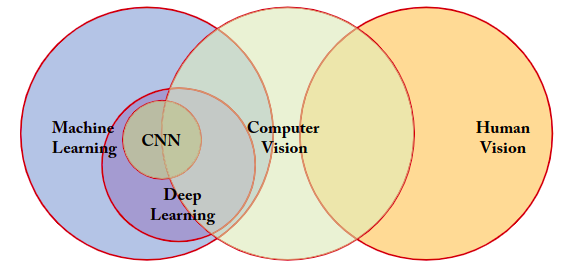
\includegraphics[width=0.6\textwidth]{images/estado_del_arte/diagrama_de_Venn_inteligencia_artificial.png}
   \caption{Relación entre Machine Learning, Deep Learning, CNN, Computer Vision y Human Vision.}
   \label{fig:diagrama_de_Venn_inteligencia_artificial}
\end{figure}

La Figura~\ref{fig:diagrama_de_Venn_inteligencia_artificial} ilustra la relación entre estos conceptos \cite{khan2018guide}. Las CNN son una subcategoría del Deep Learning, que a su vez es una subcategoría del Machine Learning. Además, las CNN están estrechamente relacionadas con la visión por computador, que busca emular la capacidad de los humanos para interpretar imágenes y vídeos.

Las CNN se inspiran en la forma en que los humanos percibimos el mundo visual. Al igual que nuestro sistema visual, que procesa la información de manera jerárquica, las CNN utilizan capas convolucionales para extraer características de bajo nivel (como bordes y texturas) y capas más profundas para identificar patrones y objetos más complejos. Esta jerarquía de características permite a las CNN aprender representaciones ricas y abstractas de los datos visuales.

La operación de convolución es fundamental en las CNN. Esta operación consiste en aplicar un filtro (o kernel) a una imagen para extraer características locales. El filtro se desliza sobre la imagen, multiplicando sus valores por los valores de la imagen en cada posición y sumando los resultados. Este proceso genera un mapa de activación que resalta las características relevantes de la imagen. 

\begin{figure}[H]
   \centering
   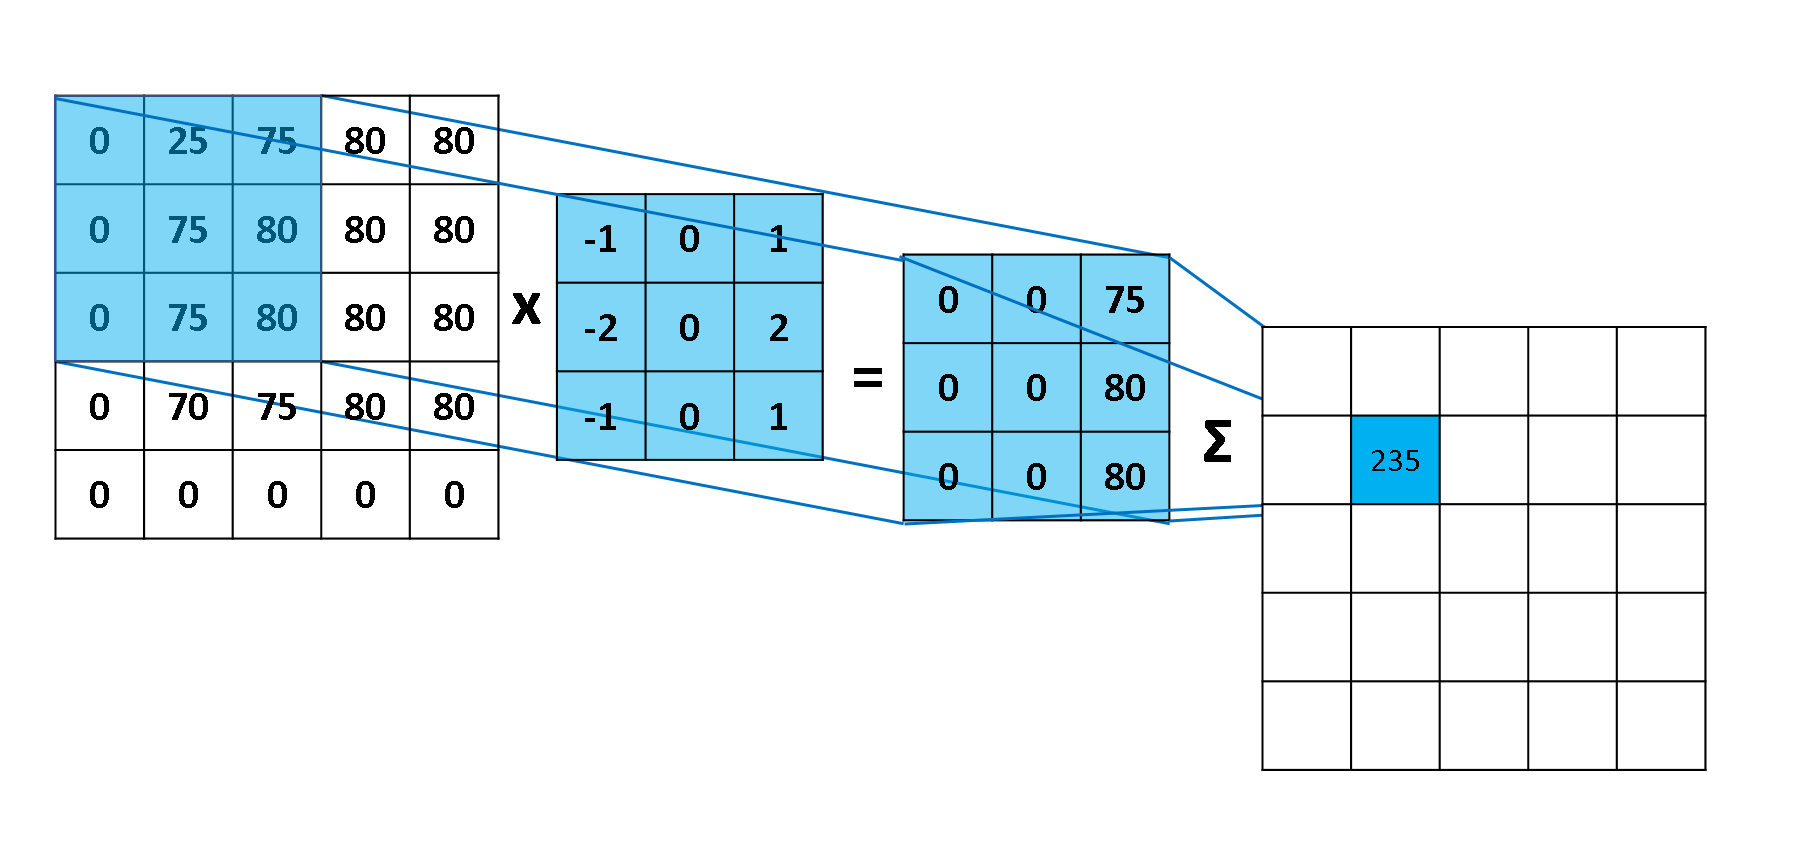
\includegraphics[width=0.6\textwidth]{images/estado_del_arte/operacion_convolucion.png}
   \caption{Operación de convolución en una imagen.}
   \label{fig:operacion_convolucion}
\end{figure}

La Figura~\ref{fig:operacion_convolucion} muestra un ejemplo de la operación de convolución. En este caso, se aplica un filtro de 3x3 a una imagen de entrada, generando un mapa de activación que resalta las características detectadas por el filtro.

\begin{figure}[H]
   \centering
   \begin{subfigure}[b]{0.25\textwidth}
      \centering
      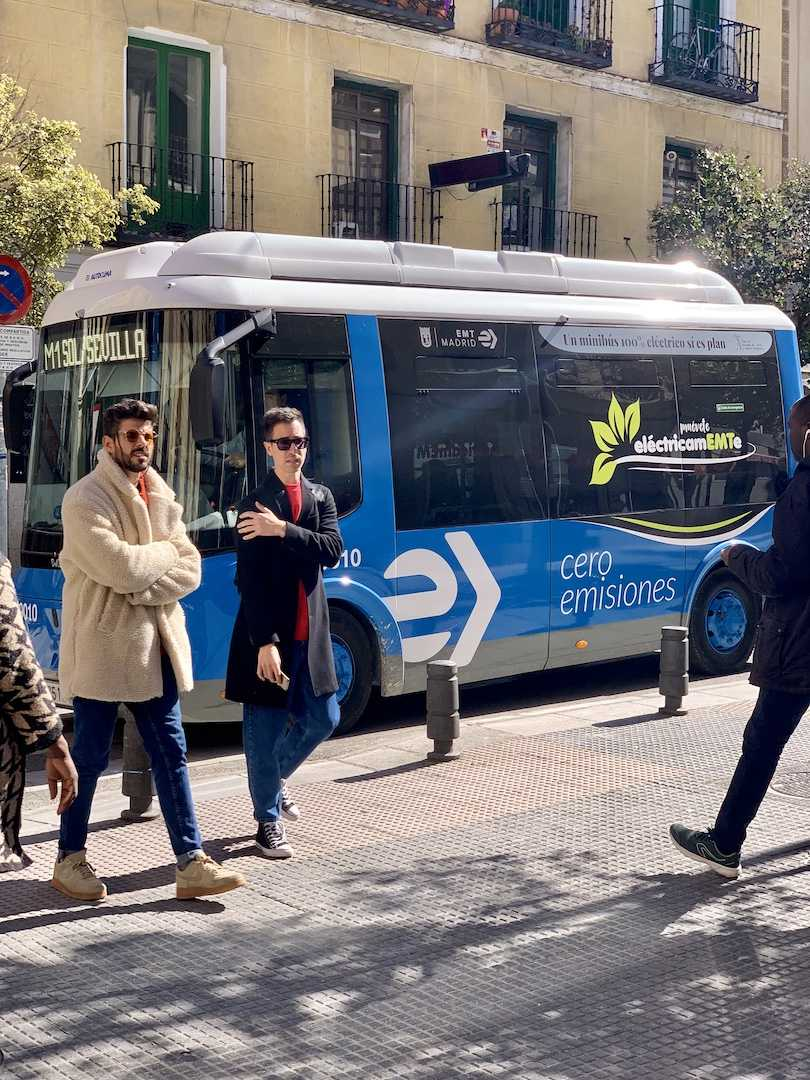
\includegraphics[width=\textwidth]{images/estado_del_arte/bus_original.jpg}
      \caption{Imagen de un autobús.}
      \label{fig:bus_original}
   \end{subfigure}
   \hfill
   \begin{subfigure}[b]{0.7\textwidth}
      \centering
      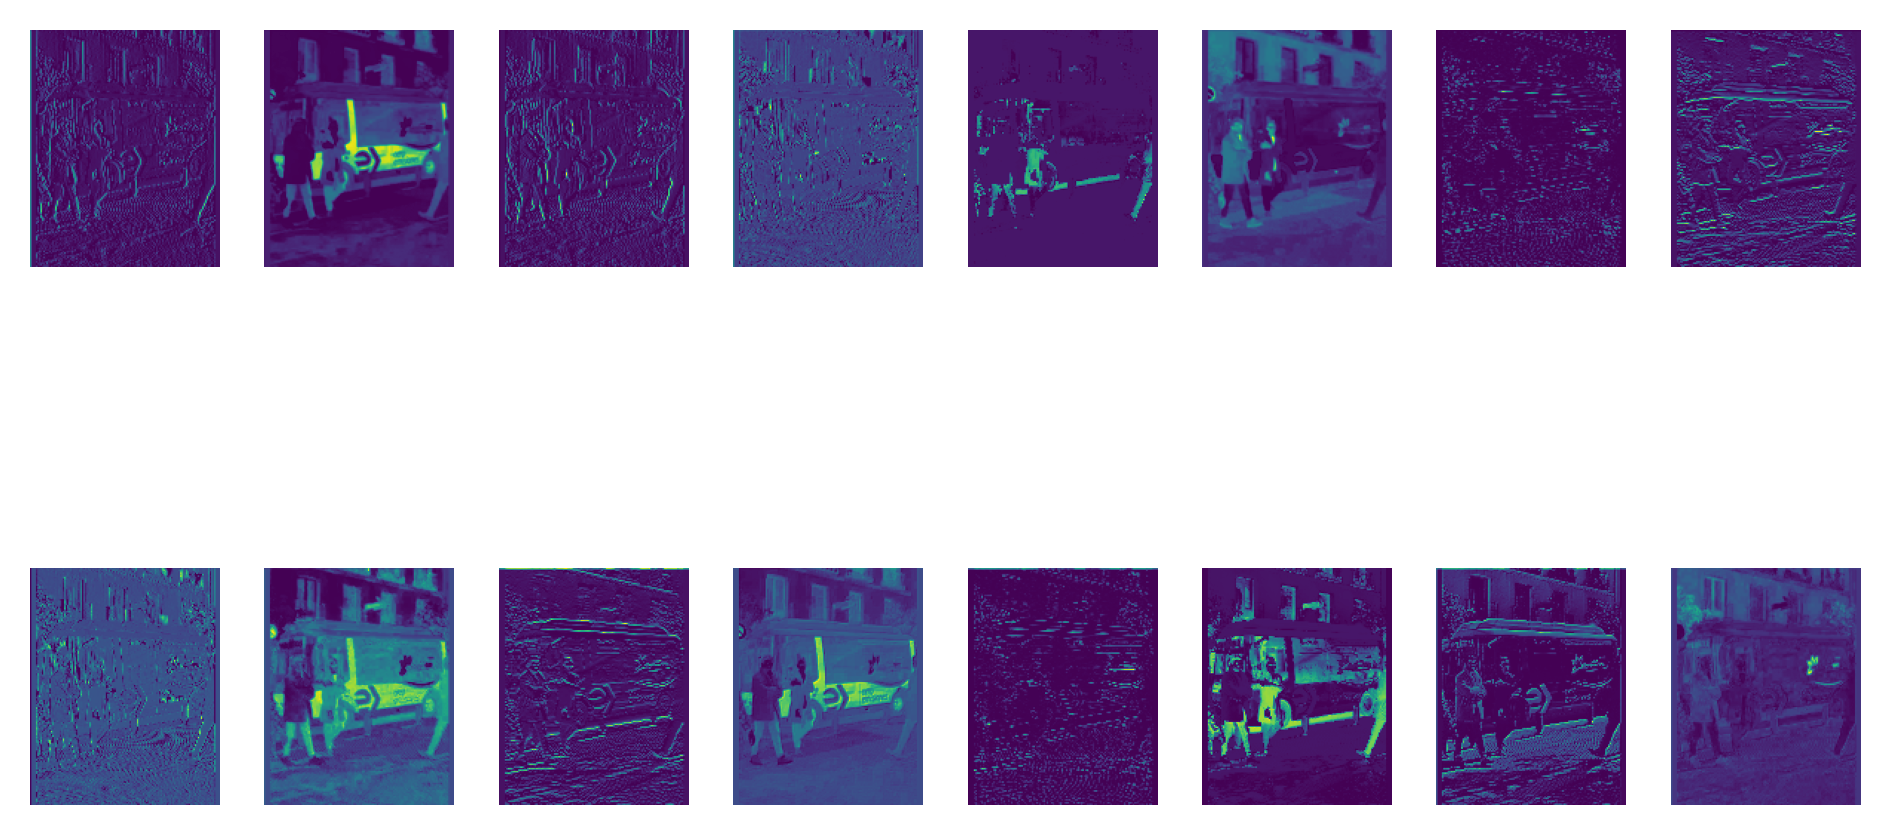
\includegraphics[width=\textwidth]{images/estado_del_arte/bus_primera_capa_convolucion.png}
      \caption{Resultado de la operación de convolución.}
      \label{fig:bus_primera_capa_convolucion}
   \end{subfigure}
   \caption{Proceso de convolución aplicado a una imagen de un autobús.}
   \label{fig:bus_convolucion}
\end{figure}

La Figura~\ref{fig:bus_convolucion} ilustra el proceso de la primera convolución del modelo yolo11n \cite{yolo11_ultralytics}. En la parte izquierda se muestra la imagen original de un autobús, mientras que en la parte derecha se presenta el resultado de aplicar la operación de convolución. En este caso, los 16 filtros de la primera capa convolucional han detectado diferentes características de la imagen, como bordes y texturas. Este proceso se repite en múltiples capas, lo que permite a la red aprender representaciones cada vez más complejas de la imagen.




\begin{enumerate}
   \item \textbf{Fundamentos del Deep Learning}
   \begin{enumerate}
      \item Concepto de aprendizaje profundo
      \item Redes neuronales artificiales básicas
      \item Función de activación, pesos y capas
   \end{enumerate}

   \item \textbf{Redes neuronales profundas}
   \begin{enumerate}
      \item Arquitecturas multicapa
      \item Desafío del desvanecimiento del gradiente
      \item Técnicas de inicialización y normalización
   \end{enumerate}

   \item \textbf{Redes neuronales convolucionales (CNN)}
   \begin{enumerate}
      \item Operación de convolución y su importancia
      \item Capas convolucionales, pooling y fully-connected
      \item Invarianza a la traslación y extracción jerárquica de características
   \end{enumerate}

   \item \textbf{Detección de objetos: primeros enfoques}
   \begin{enumerate}
      \item Sliding window
      \item Uso de características handcrafted (HOG, SIFT)
      \item Limitaciones de los enfoques tradicionales
   \end{enumerate}

   \item \textbf{Detectores de dos etapas (two-stage)}
   \begin{enumerate}
      \item R-CNN: region proposals + clasificación
      \item Fast R-CNN: mejoras compartiendo cálculos
      \item Faster R-CNN: Region Proposal Network (RPN)
      \item Mask R-CNN: incorporación de segmentación
   \end{enumerate}

   \item \textbf{Detectores de una etapa (one-stage)}
   \begin{enumerate}
      \item SSD (Single Shot MultiBox Detector)
      \item RetinaNet y Focal Loss
      \item Ventajas en velocidad vs. precisión
   \end{enumerate}

   \item \textbf{YOLO (You Only Look Once)}
   \begin{enumerate}
      \item YOLOv1: división en grid y predicción directa
      \item YOLOv2/YOLO9000: mejoras con anchor boxes
      \item YOLOv3: múltiples escalas y características
      \item YOLOv4: mejoras en backbone y técnicas de aumento
   \end{enumerate}

   \item \textbf{Evolución reciente de YOLO}
   \begin{enumerate}
      \item YOLOv5: optimización y escalabilidad
      \item YOLOv6/v7: avances arquitectónicos
      \item YOLOv8: modularidad y rendimiento
      \item YOLO11: nuevas características y optimizaciones
   \end{enumerate}

   \item \textbf{Métricas de evaluación}
   \begin{enumerate}
      \item Precisión y recall
      \item IoU (Intersection over Union)
      \item mAP50 y mAP50-95
      \item Velocidad (FPS) y compromiso velocidad-precisión
   \end{enumerate}
\end{enumerate}


\section{Aceleradores de procesamiento gráfico}
Evolución de los aceleradores de procesamiento gráfico desde la GPU, hasta los dispositivos de bajo consumo en la serie Jetson de NVIDIA.
Comentar también TensorRT y como se utiliza para optimizar los modelos en inferencias para los dispositivos de NVIDIA.

\section{Seguimiento de objetos en tiempo real}
Explicación de como funcionan los algoritmos de multi-object tracking (MOT) en tiempo real, filtro de Kalman hasta BYTETrack.

\section{Slicing Aided Hyper Inference}
Explicación de la técnica de Slicing Aided Hyper Inference, como se utiliza para mejorar la precisión de los modelos de detección de objetos y como se aplica en este trabajo.

\chapter{Análisis del problema}

????? ????????????? ????????????? ????????????? ????????????? ????????????? 

\chapter{Diseño e implementación de la solución}
En este capítulo se explicará la solución propuesta, como se ha diseñado y como se ha implementado.

\section{Descripción del sistema}

Descripción del sistema de visión artificial propuesto, como se ha diseñado y como se ha implementado.

\section{Diseño de las etapas del sistema}

Descripción de las etapas del sistema, como se han diseñado y como se han implementado.

Etapas del sistema:
\begin{itemize}
   \item \textbf{Captura de imágenes:} Descripción de la etapa de captura de imágenes, como se ha diseñado y como se ha implementado.
   \item \textbf{Inferencia:} Descripción de la etapa de inferencia, como se ha diseñado y como se ha implementado.
   \item \textbf{Seguimiento:} Descripción de la etapa de seguimiento, como se ha diseñado y como se ha implementado.
   \item \textbf{Escritura de resultados:} Descripción de la etapa de escritura de resultados, como se ha diseñado y como se ha implementado.
\end{itemize}

\section{Segmentación de las etapas del sistema}

Tipos de segmentación de las etapas del sistema:

\begin{itemize}
   \item \textbf{No segmentada:} Secuencial
   \item \textbf{Segmentación basada en hilos:} Cada etapa del sistema se ejecuta en un hilo diferente.
   \item \textbf{Segmentación basada en procesos:} Cada etapa del sistema se ejecuta en un proceso diferente.
   \item \textbf{Segmentación basada en hardware:} La etapa de inferencia se ejecuta en GPU, DLA0 y DLA1.
   \item \textbf{Segmentación basada en procesos con memoria compartida:} Cada etapa del sistema se ejecuta en un proceso diferente, pero comparten la memoria.
\end{itemize}
    


\chapter{Análisis de la solución}

En este capítulo se analizará la solución propuesta variando los parámetros posibles

\section{Variación de los parámetros}
Explicación de los parámetros que se pueden variar en la solución propuesta y su efecto en el rendimiento del sistema.

------PRUEBA--------


\begin{table}[h]
   \centering
   \resizebox{\textwidth}{!}{ % Ajusta el ancho al tamaño de la página
   \pgfplotstabletypeset[
       col sep=comma, % Definir separador de columnas (por si el CSV usa comas)
       header=true,    % Usar la primera línea como encabezado
       columns={Model, IoU, CPU_Inference, GPU_Inference, DLA_Inference, CPU_Power, GPU_Power, DLA_Power, CPU_Energy, GPU_Energy, DLA_Energy}, % Seleccionar columnas a mostrar
       display columns/0/.style={column name=Model, string type}, % Formato de la columna 'Model'
       display columns/1/.style={column name=IoU}, % Formato de la columna 'IoU'
       display columns/2/.style={column name=CPU\_Inference, column type={|c|}}, % Estilo para columnas de inferencia
       display columns/3/.style={column name=GPU\_Inference, column type={|c|}}, 
       display columns/4/.style={column name=DLA\_Inference, column type={|c|}},
       display columns/5/.style={column name=CPU\_Power, column type={|c|}}, % Estilo para columnas de potencia
       display columns/6/.style={column name=GPU\_Power, column type={|c|}},
       display columns/7/.style={column name=DLA\_Power, column type={|c|}},
       display columns/8/.style={column name=CPU\_Energy, column type={|c|}}, % Estilo para columnas de energía
       display columns/9/.style={column name=GPU\_Energy, column type={|c|}},
       display columns/10/.style={column name=DLA\_Energy, column type={|c|}},
       every head row/.style={before row=\toprule, after row=\midrule}, % Reglas horizontales en el encabezado
       every last row/.style={after row=\bottomrule}, % Reglas horizontales al final
       every column/.style={sci zerofill}, % Opcional, ajusta el formato numérico
       empty cells with={NaN} % Reemplaza celdas vacías o con guiones por NaN
   ]{excels/model_comparasion.csv} % Aquí pones la ruta del archivo CSV
   }
   \caption{Comparación de modelos en términos de inferencia, consumo de energía y potencia.}
   \label{tab:model_comparasion}
\end{table}



------PRUEBA--------



\section{Tipo de segmentación}
En esta sección se analizará el rendimiento de la solución propuesta variando el tipo de segmentación de las etapas del sistema con gráficas y tablas.

\section{Talla del modelo}
En esta sección se analizará el rendimiento de la solución propuesta variando la talla del modelo de detección de objetos con gráficas y tablas.

\section{Precisión del modelo}
En esta sección se analizará el rendimiento de la solución propuesta variando la precisión del modelo de detección de objetos con gráficas y tablas.

\section{Modo de energía y cores de la CPU}
En esta sección se analizará el rendimiento de la solución propuesta variando el modo de energía del dispositivo y el número de cores de la CPU con gráficas y tablas.

\section{Tamaño de la imagen}
En esta sección se analizará el rendimiento de la solución propuesta variando el tamaño de la imagen de entrada del modelo con la técnica de Slicing Aided Hyper Inference (SAHI) con gráficas y tablas.

\chapter{Prueba de concepto}
Aqui se explicará la implementación de la solución propuesta en el entorno de producción con la cinta transportadora.

\section{Construcción del entorno}

\section{Instalación del entorno}






????? ????????????? ????????????? ????????????? ????????????? ?????????????


%%%%%%%%%%%%%%%%%%%%%%%%%%%%%%%%%%%%%%%%%%%%%%%%%%%%%%%%%%%%%%%%%%%%%%%%%%%%%%%
%                                 CONCLUSIONS                                 %
%%%%%%%%%%%%%%%%%%%%%%%%%%%%%%%%%%%%%%%%%%%%%%%%%%%%%%%%%%%%%%%%%%%%%%%%%%%%%%%

\chapter{Conclusiones}

????? ????????????? ????????????? ????????????? ????????????? ????????????? 

%%%%%%%%%%%%%%%%%%%%%%%%%%%%%%%%%%%%%%%%%%%%%%%%%%%%%%%%%%%%%%%%%%%%%%%%%%%%%%%
%                                BIBLIOGRAFIA                                 %
%%%%%%%%%%%%%%%%%%%%%%%%%%%%%%%%%%%%%%%%%%%%%%%%%%%%%%%%%%%%%%%%%%%%%%%%%%%%%%%

\bibliographystyle{plain}      % Estilo de la bibliografía
\bibliography{referencias} % Bibliografia

% \begin{thebibliography}{10}

% %%%%%%%%%%%%%%%%%%%%%%%%%%%%%%%%%%%%%%%%%%%%%%%%%%%%%%%%%%%%%%%%%%%%%%%%%%%%%%%
% % MODEL D'ARTICLE                                                             %
% %%%%%%%%%%%%%%%%%%%%%%%%%%%%%%%%%%%%%%%%%%%%%%%%%%%%%%%%%%%%%%%%%%%%%%%%%%%%%%%
% \bibitem{light}
%    Jennifer~S. Light.
%    \newblock When computers were women.
%    \newblock \textit{Technology and Culture}, 40:3:455--483, juliol, 1999.

% %%%%%%%%%%%%%%%%%%%%%%%%%%%%%%%%%%%%%%%%%%%%%%%%%%%%%%%%%%%%%%%%%%%%%%%%%%%%%%%
% % MODEL DE LLIBRE                                                             %
% %%%%%%%%%%%%%%%%%%%%%%%%%%%%%%%%%%%%%%%%%%%%%%%%%%%%%%%%%%%%%%%%%%%%%%%%%%%%%%%
% \bibitem{ifrah}
%    Georges Ifrah.
%    \newblock \textit{Historia universal de las cifras}.
%    \newblock Espasa Calpe, S.A., Madrid, sisena edició, 2008.

% %%%%%%%%%%%%%%%%%%%%%%%%%%%%%%%%%%%%%%%%%%%%%%%%%%%%%%%%%%%%%%%%%%%%%%%%%%%%%%%
% % MODEL D'URL                                                                 %
% %%%%%%%%%%%%%%%%%%%%%%%%%%%%%%%%%%%%%%%%%%%%%%%%%%%%%%%%%%%%%%%%%%%%%%%%%%%%%%%
% \bibitem{WAR}
% Comunicat de premsa del Departament de la Guerra, 
% emés el 16 de febrer de 1946. 
% \newblock Consultat a 
% \url{http://americanhistory.si.edu/comphist/pr1.pdf}.

% \end{thebibliography}
\cleardoublepage

%%%%%%%%%%%%%%%%%%%%%%%%%%%%%%%%%%%%%%%%%%%%%%%%%%%%%%%%%%%%%%%%%%%%%%%%%%%%%%%
%                           APÈNDIXS  (Si n'hi ha!)                           %
%%%%%%%%%%%%%%%%%%%%%%%%%%%%%%%%%%%%%%%%%%%%%%%%%%%%%%%%%%%%%%%%%%%%%%%%%%%%%%%

\APPENDIX

%%%%%%%%%%%%%%%%%%%%%%%%%%%%%%%%%%%%%%%%%%%%%%%%%%%%%%%%%%%%%%%%%%%%%%%%%%%%%%%
%                         LA CONFIGURACIO DEL SISTEMA                         %
%%%%%%%%%%%%%%%%%%%%%%%%%%%%%%%%%%%%%%%%%%%%%%%%%%%%%%%%%%%%%%%%%%%%%%%%%%%%%%%

\chapter{Configuración del sistema}

????? ????????????? ????????????? ????????????? ????????????? ?????????????

\section{Fase de inicialitzación}

????? ????????????? ????????????? ????????????? ????????????? ?????????????

\section{Identificación de dispositivos}

????? ????????????? ????????????? ????????????? ????????????? ?????????????

%%%%%%%%%%%%%%%%%%%%%%%%%%%%%%%%%%%%%%%%%%%%%%%%%%%%%%%%%%%%%%%%%%%%%%%%%%%%%%%
%                               ALTRES  APÈNDIXS                              %
%%%%%%%%%%%%%%%%%%%%%%%%%%%%%%%%%%%%%%%%%%%%%%%%%%%%%%%%%%%%%%%%%%%%%%%%%%%%%%%


\chapter{??? ???????????? ????}

????? ????????????? ????????????? ????????????? ????????????? ????????????? 



%%%%%%%%%%%%%%%%%%%%%%%%%%%%%%%%%%%%%%%%%%%%%%%%%%%%%%%%%%%%%%%%%%%%%%%%%%%%%%%
%                              FI DEL DOCUMENT                                %
%%%%%%%%%%%%%%%%%%%%%%%%%%%%%%%%%%%%%%%%%%%%%%%%%%%%%%%%%%%%%%%%%%%%%%%%%%%%%%%

\end{document}
